% !TEX TS-program = pdflatex
% !TEX encoding = UTF-8 Unicode

% This is a simple template for a LaTeX document using the "article" class.
% See "book", "report", "letter" for other types of document.

\documentclass[12pt]{report} % use larger type; default would be 10pt

\usepackage[utf8]{inputenc} % set input encoding (not needed with XeLaTeX)

%%% Examples of Article customizations
% These packages are optional, depending whether you want the features they provide.
% See the LaTeX Companion or other references for full information.

%%% PAGE DIMENSIONS
\usepackage{geometry} % to change the page dimensions
\geometry{a4paper} % or letterpaper (US) or a5paper or....
% \geometry{margin=2in} % for example, change the margins to 2 inches all round
% \geometry{landscape} % set up the page for landscape
%   read geometry.pdf for detailed page layout information

\usepackage{graphicx} % support the \includegraphics command and options

% \usepackage[parfill]{parskip} % Activate to begin paragraphs with an empty line rather than an indent

%%% PACKAGES
\usepackage{booktabs} % for much better looking tables
\usepackage{array} % for better arrays (eg matrices) in maths
\usepackage{paralist} % very flexible & customisable lists (eg. enumerate/itemize, etc.)
\usepackage{verbatim} % adds environment for commenting out blocks of text & for better verbatim
\usepackage{subfig} % make it possible to include more than one captioned figure/table in a single float
\usepackage[final]{pdfpages}
% These packages are all incorporated in the memoir class to one degree or another...

%%% HEADERS & FOOTERS
\usepackage{fancyhdr} % This should be set AFTER setting up the page geometry
\pagestyle{fancy} % options: empty , plain , fancy
\renewcommand{\headrulewidth}{0pt} % customise the layout...
\lhead{}\chead{}\rhead{}
\lfoot{}\cfoot{\thepage}\rfoot{}

%%% SECTION TITLE APPEARANCE
\usepackage{sectsty}
\allsectionsfont{\sffamily\mdseries\upshape} % (See the fntguide.pdf for font help)
% (This matches ConTeXt defaults)

%%% RULE

\newcommand{\HRule}{\rule{\linewidth}{0.5mm}}

%%% BIBLIOGRAPHY

\usepackage{apacite}                           %bibliography in apa-style

%%% ToC (table of contents) APPEARANCE
\usepackage[nottoc,notlof,notlot]{tocbibind} % Put the bibliography in the ToC
\usepackage[titles,subfigure]{tocloft} % Alter the style of the Table of Contents
\renewcommand{\cftsecfont}{\rmfamily\mdseries\upshape}
\renewcommand{\cftsecpagefont}{\rmfamily\mdseries\upshape} % No bold!

\setcounter{secnumdepth}{-2}

%%% END Article customizations

%%% The "real" document content comes below...

\begin{document}

\begin{titlepage}

\begin{center}


% Upper part of the page

\includegraphics[width=1\textwidth]{./logo}\\[1cm]    

\textsc{\Large Bachelor Thesis}\\[0.5cm]
\textsc{\Large {[}201000166{]}}\\[0.5cm]


% Title
\HRule \\[0.4cm]
{ \huge \bfseries Research Proposal}\\[0.4cm]

\HRule \\[1.5cm]

% Author and supervisor
\begin{minipage}{0.4\textwidth}
\begin{flushleft} \large
\emph{Author:}\\
Micha \textsc{van den Enk} \\
{[}s1004654{]} \\
\end{flushleft}
\end{minipage}
\begin{minipage}{0.4\textwidth}
\begin{flushright} \large
\emph{Supervisors:} \\
Dr. H. H. \textsc{Leemkuil} \\
Second \textsc{supervisor} \\
\end{flushright}
\end{minipage}

\vfill

% Bottom of the page
{\large DATE}

\end{center}

\end{titlepage}

\tableofcontents

\chapter{Preface}

In this document the reader can find a proposal for designing a course on quantum mechanics in a qCraft learning environment. This is an assignment executed for a bachelor thesis. The document contains a table with general information, a short summary of the assignment, a detailed description of the assignment wth the rationale, the conceptual framework and the relevance, the design approach and a planning.

\chapter{General Information}

\begin{center}
\begin{tabular}{ l p{8cm} }
Researcher & Micha van den Enk (s1004654) \\
Study & Onderwijskunde \\
Study Department & Instructional Technology \\ 
Date & \\
First supervisor & Dr H. H. Leemkuil \\
Second supervisor & \\
Keywords & Quantum mechanics, Middle school Education, Netherlands \\
Title & \\
\end{tabular}
\end{center}

\chapter{Summary}

\chapter{Description}

This chapter contains a short description of the background of the subject matter on middle schools in the Netherlands, the content of the instruction itself, the technology which will be used for the instruction, and an outline conceptual framework for the literature study.

\section{Background}

In the Netherlands, quantum mechanics always used to be a topic which schools themselves could choose to teach or not to teach. The only skill students had to know for the Centraal Eindexamen (the national central exams at the end of high school) which comes close to quantum mechanics is to elucidate the photoelectric and the wave-particle duality, mentioned within point 20 under subdomain E3 (citation eindexamenblad). However, one of the changes in the Centraal Eindexamen of 2016 was the addition of domain F1, which is called Quantum world. For this subdomain the candidate has to be able to apply the wave-particle duality and the uncertainty principle of Heisenberg, and to explain the quantization of energy levels in some examples with a simple quantum physical model. In order to give all candidates a chance of passing this subdomain, schools have to alter their programs in order to meet the expectations of the Centraal Eindexamen.

However, when searching the internet using the search machine Google concerning the implementation of quantum mechanics in Dutch high schools, the quantity and the quality of the results are very low. There are also no results to be found in the Dutch papers. An example is the Dutch site http://www.quantumuniverse.nl/, where teachers can find a small amount of brief courses on fundamental quantum mechanics, and where the forums are very quiet with only 5 discussions, of which 4 are just started threads from the site administrator.

Upon finding this information, an expert was consulted to confirm this conjecture. The expert was researching the implementation of quantum mechanics on middle schools, and she also a first degree physics teacher. She stated that within her school there were no initiatives to bring this topic in their classrooms, and that their school was no exception as well.

The fact that next year domain F1 has to be fully implemented and teached to all vwo students who chose physics as an examination subject is therefore slowly turning into a sword of Damocles. This stresses the urgency for the development of new course material.

\section{Content}

Quantum is not the most easy topic to introduce to physics. The subject is very counterintuitive, and still poses headaches to many physicists today. The great physicist Richard Feynman is known for saying: “I think I can safely say that nobody understands quantum mechanics” (1965), and this statement still holds. Quantum mechanics is this counterintuitive because it contradicts a lot of axioms we inherited from classical physics. These contradictions are highlighted by an article written by Einstein, Podolsky and Rosen, which states that the current understanding of quantum mechanics contradict the criterion of reality and the hypothesis of locality.

There are a lot of resources available for teaching quantum mechanics. Most of these resources are academical and focus on teaching the mathematics. Their philosophy is that the student can only really get a grasp on quantum mechanics if he understand the underlying mathematical mechanics. An example of such a resource is \citeA{qumech}. These resources are not very usefull when teaching middle school students, because it demands an understanding of mathematics which is beyond the knowledge of middle school students, for example the integration of Schröder equations.

The other way of teaching quantum mechanics is by teaching the key principles of quantum mechanics. A fashion in which this could be achieved is by only considering the perfectly correlating instances. An example of such an instance is quantum teleportation. \citeA{dance} explains this phenomenon without having to resort to very complex mathematics, but still explaining the fundamentals of quantum mechanics, namely observer dependency, superposition and quantum entanglement. The instruction will therefore use quantum teleportation to explain these three fundamental principles, so the learner will gain a concepual understanding of quantum mechanics.

\section{Technology}

The course will make use of qCraft, a modification made by members of Google for the game Minecraft. This game supports an accessible way for the player to get introduced and to interact with the aforementioned principles superposition, observer dependency and entanglement.

\subsection{Minecraft}



\section{Conceptual framework}

\chapter{Design approach}

A model which describes the process of developing educational resources is the Generic Model \cite{genericmodel} (see figure~\ref{fig:genmod}). It describes the phases Analysis, Design, Development, Implementation and Evaluation. This model will be partly used for this project. Because of time constraints and the limited size of the project it will only go as far as the horizontal bar of development, this will be elaborated further later in this chapter.

\begin{figure}[h]
\centering
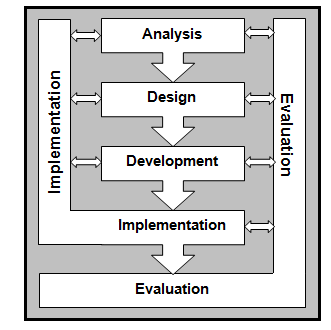
\includegraphics[width=0.7\textwidth]{genericmodel}
\caption{\footnotesize The generic model by \protect\citeA{genericmodel}\label{fig:genmod}}
\end{figure}

\section{Analyses}

The first step in the Generic Model \cite{genericmodel} is the step Analysis. In this step, data is gathered which is necessary for designing an effective solution. \citeA{smithragan} mention three different kinds of analysis, namely analyzing the learning context, analyzing the learners and analyzing the learning task.

\subsection{Analyzing the learning context}

A learning task always takes place in a certain learning context. In this case this is the middle school. It entails not only the place, but also the temporal and social environment \cite{smithragan}. The analysis of the learning context can provide the instructional needs and a description of the different factors influencing the instruction. With the instructional needs, the designer can establish the main learning goals for the instruction. The description of the learning environment can provide the learning opportunities and constraints which have to be taken into account for the instruction.

\subsection{Analyzing the learners}

The second analysis is that of the learners \cite{smithragan}. The purpose of this analysis is the characterization of the end user of the instruction, which is in this case the middle school students. For this analysis it is important to determine the similarities and differences between the learners. \citeA{smithragan} provide a list of factors which play a role in designing the instruction.

\subsection{Analyzing the learning task}

The final step is analyzing the learning task \cite{smithragan}. In this analysis the goals from the needs assessment during the analysis of the learning context have to be translated to test specifications, with which the content of the instruction can be established. In order to achieve these test specifications, first the type of learning has to be established. Having this established, the information-processing analysis can be conducted. Every type of learning has its own kind of information-processing analysis. \citeA{dance} will be used to conduct this information-processing analysis. The next step is the prerequisite analysis. The outcome of this has to correspond to the outcome of the learner analysis. Finally, the learning objectives can be written, which form the test specifications. Every learning objective has to contain a description of the terminal behavior or actions that will demontsrate learning, a description of the conditions of demonstration of that action and a description of the standard or criterion \cite{smithragan}. Every learning objective will fall into a catagory of Bloom his taxanomy of learning objectives \cite{bloom}, and will use appropriate action verbs.

\section{Literature Study}

After the analyses have been conducted, the literature study will take place. \citeA{lerencomm} state the different steps which go into doing literature research and writing the theoretic framework. The first step of the literature study will be considering the search terms. For this, the results of the analyses will have to be taken into account, especially the characterizations of the learners and the learning task. The search terms will then be expanded by finding synonyms and similar relevant terms by using the Thesaurus. After the search terms are determined, it has to be established which databases will provide useful results. Then a cyclic process will take place in which the amount of results will be assessed with these databases and search terms and then if needed the results are limited or expanded by using more search terms and filters. The results will always be constrained to peer-reviewed articles. Other filters could than be the recency of the articles or the educational level of the test subjects. When there is an appropriate amount of results, they will be filtered manually. First, the articles which seem relevant by their title and keywords will be selected. This will be done in a very broad sense, so only the really irrelevant results will be filtered out. These selected articles will then be skimmed by their abstract, introduction and conclusion and will be filtered out when they actually are not relevant. The remaining articles will then be used for constructing the theoretic framework. It could be that new keywords can be found in these articles. In this case this keyword will be added to the search terms in order to find even more results.

From the resulting articles a literature matrix will be constructed \cite{lerencomm}. This matrix will contain research questions in the top row and the resulting articles in the left row. By using this technique, every question can be answered per resulting article. The columns can then be summarized in order to answer every question separately. These answers ultimately are the content of the theoretic framework.

\section{Design}

The second phase of the Generic Model \cite{genericmodel} is the design phase. In this phase the results from the analyses are used to form design principles, which can be used to develop the instruction. There will be design principles for:
\begin{itemize}
\item a pretest for information about the preknowledge and the experience with playing games of the participants;
\item the text of the instruction;
\item the learning environment within Minecraft;
\item the posttest for testing the resulting knowledge of the participants.
\end{itemize}
Furthermore, a global design plan will be made, which is a distribution of the learning objectives over the course of the instruction. The basic hierarchy of the instruction will consist of the different learning events by \citeA{smithragan}.

\section{Development}

After the design phase comes the development phase, in which all the resources are finally fully developed, based on the earlier made design. This will be the developing of the pre- and posttest, the writing of the text and the developing of the learning environment in Minecraft. The development of the resources will be based on the earlier developed design principles and the global design plan.

\section{Formative Evalutation}

After the first development phase, the formative evaluations will take place. These evaluations are derived from the \emph{Evaluation Matchboard} \cite{evamatchboard}. After each evaluation, adjustments of the products have to take place as well. First, the resources will be screened to check whether the resources confirm to the design principles. Then, a focus group evaluation will take place. In this evaluation a subject matter expert will be interviewed to check whether the text contains statements which have to be adjusted or corrected with the current knowledge on quantum teleportation. Finally, a micro-evaluation will take place, in which the final product will be tested upon members of the target audience, or people similar to the target group audience. With this evaluation, the actual practicality can be tested by interviewing the participants. The actual effectiveness will also be tested by letting the participants make the posttest.

\section{Implementation and Summative Evaluation}

The implementation and summative evaluation will not take place during this project. Implementation would be outside of the scope of the project, and could only be executed in a follow-up project. When proven to be succesful, the resources developed will be offered to MinecraftEdu, an organisation which has the mission to bring Minecraft into schools.

Because the lack of implementation, a summative evaluation is also out of the question. In order to conduct a succesful summative evaluation, the resources would have to be fully in use in the actual context, which is not the case for this project.

\section{Conclusion and Discussion}

When the micro-evaluation has taken place, the resulting data has to be processed and analyzed. With these results, a conclusion will be written down to summarize the advantages and drawbacks of the instruction. There also will be suggestions for improvement and for implementation.

\chapter{Planning}

\begin{center}
\begin{tabular}{ l r }
Analyses & Week 18 \\
Literature research & Week 20 \\
Design & Week 21 \\
Development & Week 22 \\
Formative Evaluation & Week 24 \\
Conclusion/Discussion & Week 25 \\
Presentation & Week 26 \\
\end{tabular}
\end{center}

\bibliographystyle{apacite}
\bibliography{references}

\part{Appendix A: Evaluation matchboard}

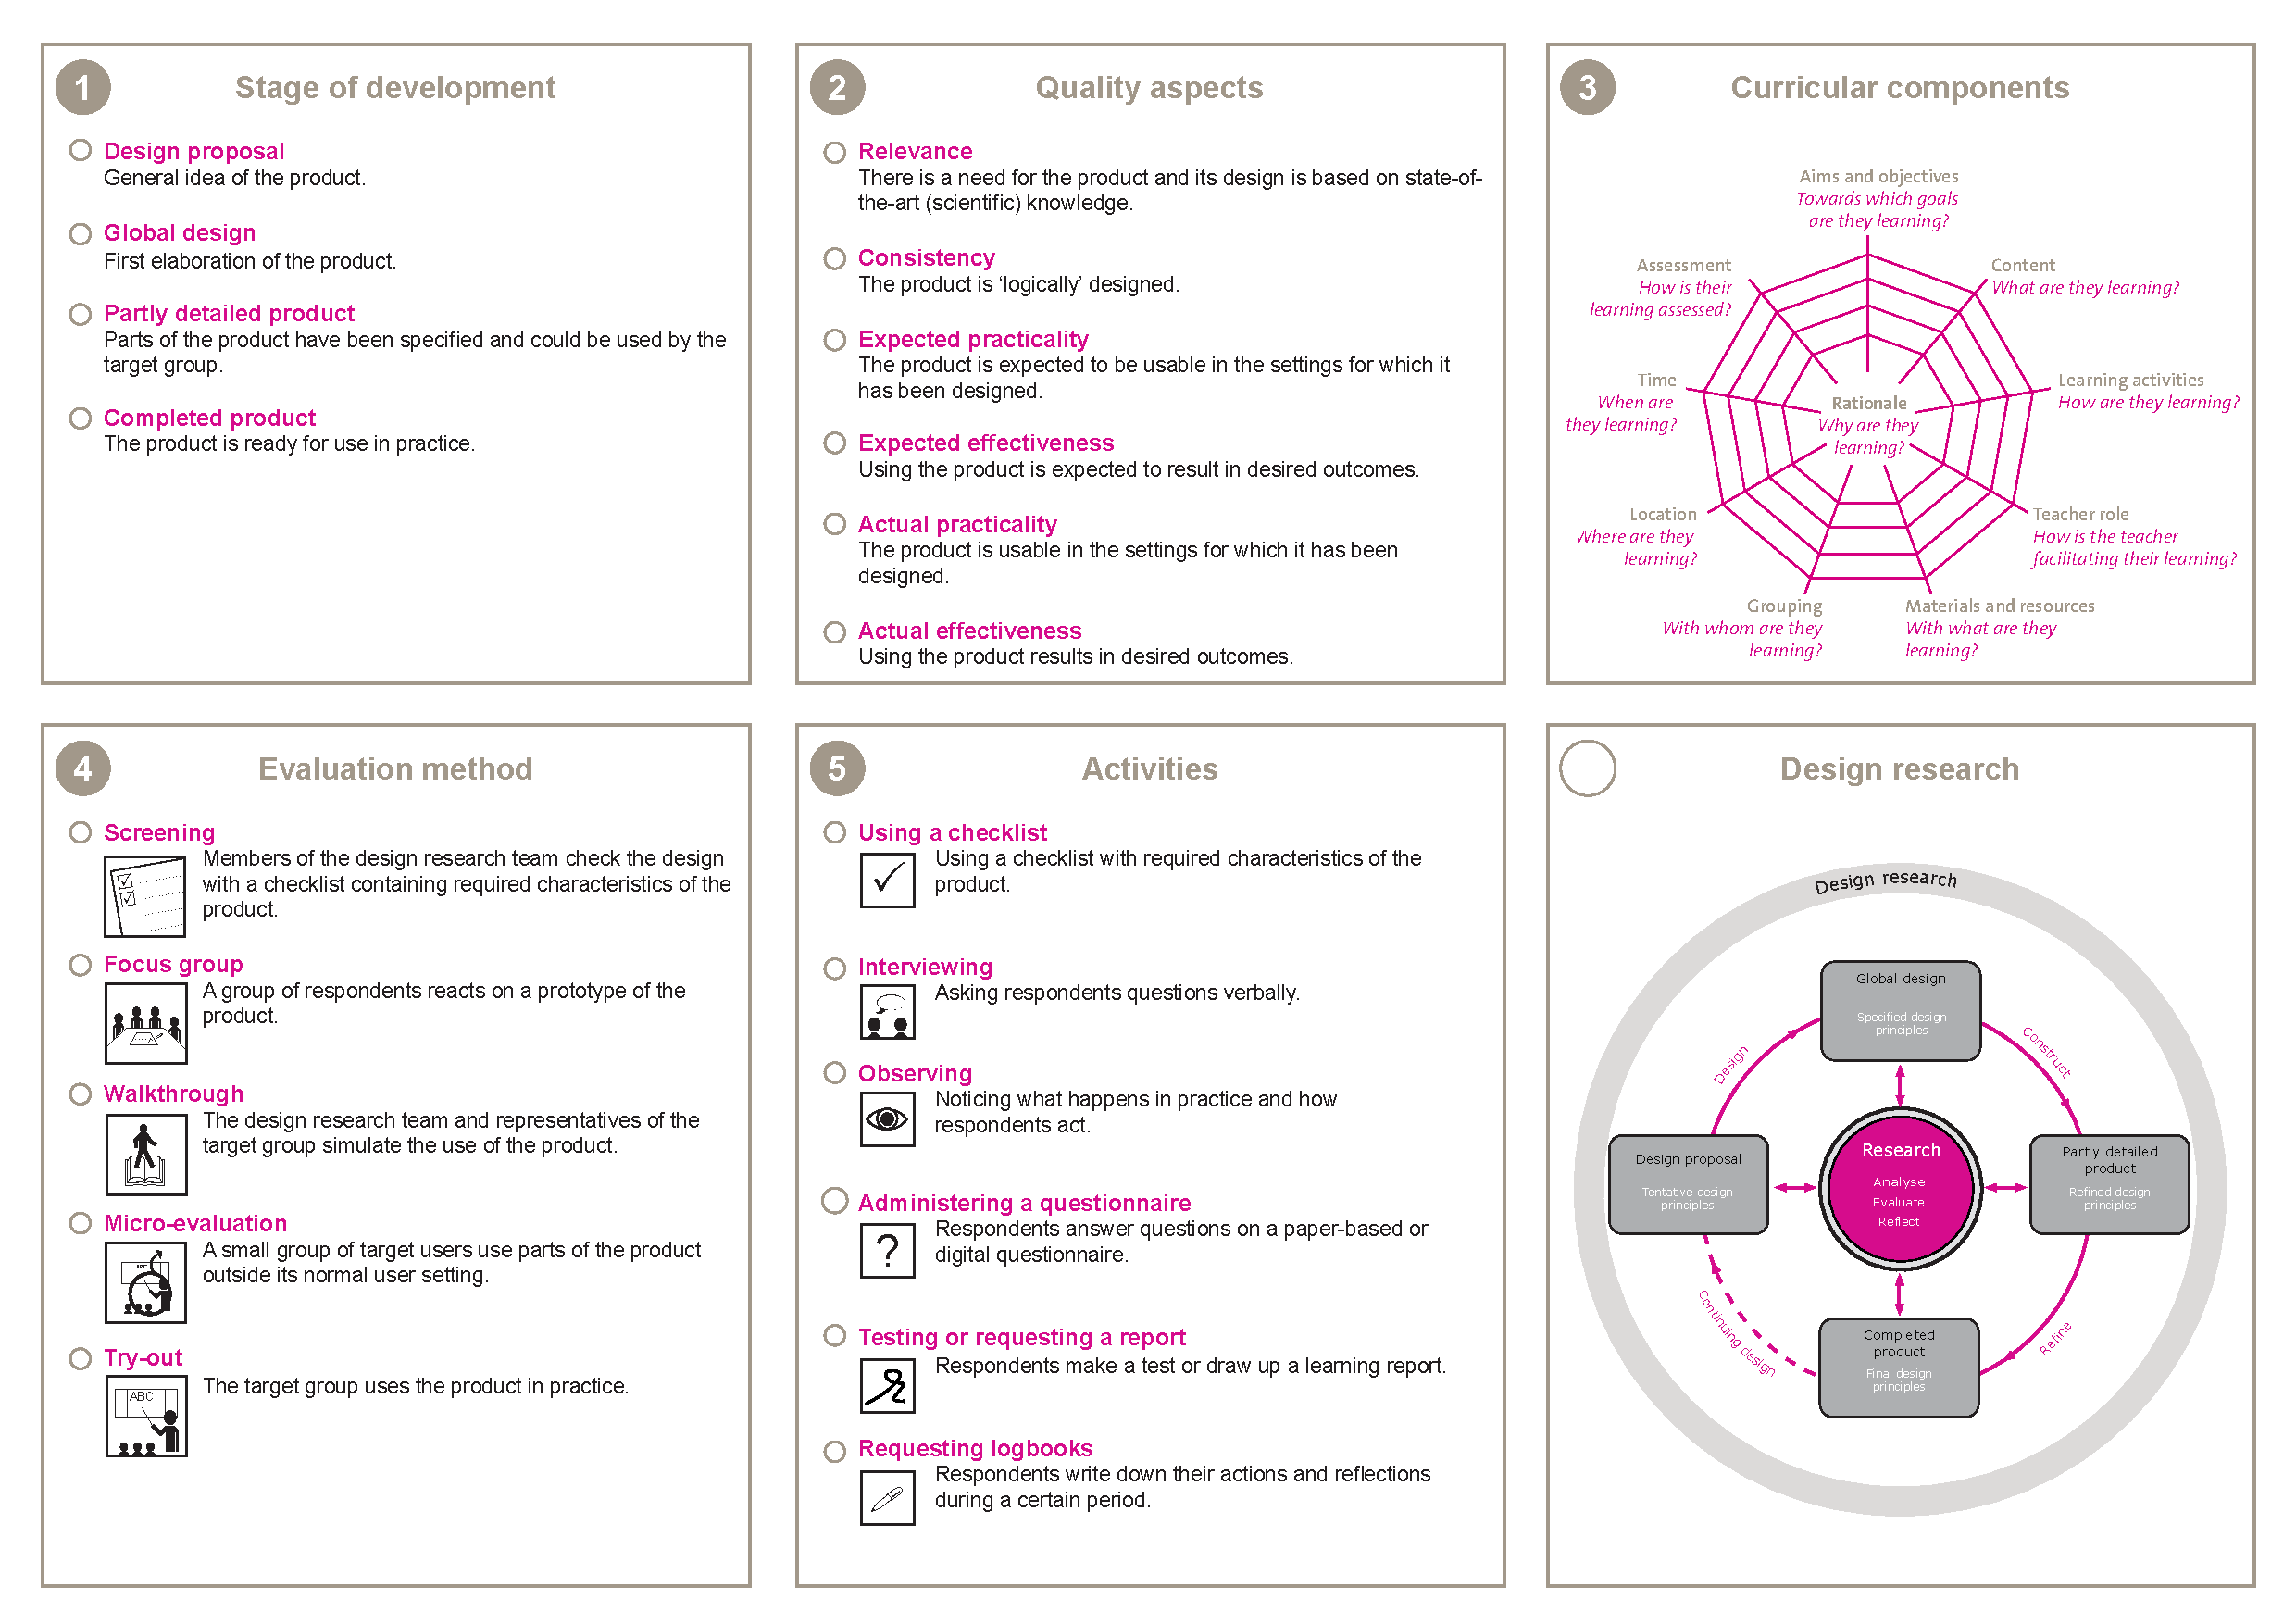
\includepdf[pages=-]{Evaluation_matchboard.pdf}

\end{document}
